\documentclass[11pt,a4paper]{article}
\usepackage[utf8]{inputenc}
\usepackage[margin=1in]{geometry}
\usepackage{amsmath, amssymb, amsfonts}
\usepackage{booktabs}
\usepackage{hyperref}
\usepackage{titlesec}
\usepackage{microtype}
\usepackage{graphicx}

% Title Configuration
\title{\textbf{Comparative Analysis of Generative Frameworks:\\ Focus on DDPM vs. Flow Matching vs. Rectified Flow}}
\author{\textbf{Presenters:} Joachim Hofmann \& Alex Hanselmann \\
\small \textbf{Context:} Master's Course in Generative Machine Learning}
\date{\textbf{Date:} May 28, 2026}

\begin{document}

\maketitle

\hrule
\vspace{0.4cm}

\section{Introduction and Research Objectives}
This report documents the findings of our research within Bundle A2 of the Generative Machine Learning curriculum\cite{87}. We address the recent paradigm shift in generative modeling: the move from stochastic diffusion processes to deterministic flow-based methods\cite{88}. While Denoising Diffusion Probabilistic Models (DDPM) established the baseline for high-fidelity synthesis, their reliance on stochastic reverse chains introduces significant computational bottlenecks\cite{89}.

Our primary mission is a comparative evaluation of DDPM, Flow Matching (FM), and Rectified Flow (RF) using the CelebA-64 dataset\cite{90}. We aim to rigorously analyze how these frameworks handle the transport from a Gaussian source to a data distribution, focusing on two research goals\cite{91}:
\begin{itemize}
    \item \textbf{Minimization of Operational Cost:} We define this through ``NFE'' (Number of Function Evaluations)---the count of neural network passes required for a single sample---and ``Wall-Clock Cost'' (Latency), the physical execution time in milliseconds (ms)\cite{91}.
    \item \textbf{Mathematical Formulation Stability:} This refers to the geometric precision of the generative trajectories\cite{92}. We quantify stability using the Mean Squared Error (MSE), which measures the ``Path Deviation'' of the model's predicted trajectory from a theoretical straight line\cite{93}.
\end{itemize}
By analyzing these metrics, we seek to demonstrate how path ``straightening'' directly impacts hardware efficiency and model stability\cite{94}.

\section{Theoretical Framework: Stochastic vs. Deterministic Transport}
The architectural divergence between these frameworks is rooted in the choice between Stochastic Differential Equations (SDE) and Ordinary Differential Equations (ODE)\cite{95}. DDPM models the generative process as a reverse-time SDE, incorporating ``stochastic jitter'' to remain stable\cite{96}. Conversely, Flow Matching and Rectified Flow utilize an ODE framework to define a smooth, deterministic velocity field\cite{97}.

\begin{table}[h]
\centering
\caption{Systematic Comparison of Generative Paradigms}
\label{tab:paradigms}
\vspace{0.2cm}
\small
\begin{tabular}{lll}
\toprule
\textbf{Dimension} & \textbf{Diffusion Models (DDPM)} & \textbf{Rectified Flow (RF)} \\
\midrule
Systemic Basis & SDE: $dx_t = f(t)x_t dt + g(t)dw_t$ & ODE: $dx_t = v(x_t, t)dt$ \\
\addlinespace
Path Interpolation & Non-linear: $X_t = \sqrt{\bar{\alpha}_t} X_1 + \sqrt{1 - \bar{\alpha}_t} \epsilon$ & Linear: $X_t = (1 - t)X_0 + tX_1$ \\
\addlinespace
Learning Target & Added Noise ($\epsilon$) & Velocity Field ($v$) \\
\addlinespace
Loss Function & $\mathcal{L} = \mathbb{E} [ \| \epsilon - \hat{\epsilon}_\theta \|^2 ]$ & $\mathcal{L} = \mathbb{E} [ \| (X_1 - X_0) - v_\theta \|^2 ]$ \\
\addlinespace
Inference Logic & Stochastic Markov Chain & Deterministic Euler Step \\
\bottomrule
\end{tabular}
\end{table}

\subsection{Path Entanglement and the Mean Value Problem}
A fundamental challenge in high-dimensional transport is ``Path Entanglement.'' Even with a linear interpolation between $X_0$ and $X_1$, different pairs of noise and data often result in crossing trajectories\cite{100}. Since a neural network $v_\theta(x, t)$ is a single-valued function, it is mathematically forced to learn the average (mean) of all target directions at any intersection point\cite{101}. This forcing leads to a time-variant, curved velocity field, which manifests empirically as ``Blur'' in generated samples and high inference costs due to the need for many small integration steps\cite{102}.

\subsection{The Mathematical Link: Eulerian vs. Lagrangian}
Flow Matching and Rectified Flow describe the same physical transport but through different lenses\cite{103}. Flow Matching typically adopts an Eulerian (Field-centric) perspective, focusing on the continuity equation\cite{104}:
\begin{equation}
\frac{\partial \rho_t(x)}{\partial t} + \nabla \cdot (\rho_t(x)v(x, t)) = 0
\end{equation}
to preserve probability mass\cite{104}. Rectified Flow adopts a Lagrangian (Particle-centric) perspective, focusing on the trajectories of individual random variable paths $X_t$\cite{105}. The goal of Rectified Flow is to solve the entanglement problem by explicitly straightening these paths\cite{106}.

\section{The Rectified Flow Framework: From Chaos to Straight Highways}
Rectified Flow provides a structured, three-phase approach to eliminate path curvature, enabling extreme inference efficiency\cite{107}.

\begin{enumerate}
    \item \textbf{Phase 1: Initial Training/Rectification (1-RF):} The model learns a velocity field $v_\theta$ to minimize the least-squares error along linear paths\cite{108}. While this establishes a valid flow, the paths still cross and curve because $X_0$ and $X_1$ are coupled independently\cite{109}.
    \item \textbf{Phase 2: The Reflow Step (2-RF):} This is the critical ``Flow-Rewiring'' phase\cite{110}. By simulating the ODE from Phase 1, we find the deterministic endpoints $X^{\text{rect}}_1$ for each $X_0$\cite{111}. This process re-pairs the noise and data to minimize the quadratic transport cost\cite{112}:
    \begin{equation}
    \min_\pi \int \|x_0 - x_1\|^2 d\pi(x_0, x_1)
    \end{equation}
    The result is a set of non-intersecting, perfectly straight trajectories\cite{112}.
    \item \textbf{Phase 3: Jump:} Once the paths are straightened and the velocity field becomes time-independent ($v(x, t) \approx v(x, 0)$), a student model $\alpha_\phi(X_0)$ is trained to predict the exact ODE endpoint $X_1$ in a single step, effectively skipping the simulation path entirely\cite{113}.
\end{enumerate}

\noindent\textbf{Analysis:} The ``Reflow'' step is what allows the generative process to collapse from many steps to one\cite{114}. By minimizing the quadratic transport cost, the model regularizes the velocity field toward homogeneity\cite{115}. This removes the necessity of an iterative solver to compensate for direction changes during inference\cite{116}.

\section{Implementation Architecture and Evaluation Metrics}
To ensure a rigorous ``fair-comparison'' environment, we utilized a routing node architecture where all models originate from a shared initial noise distribution $\mathcal{N}(0, \mathbf{I})$\cite{117}.

\subsection{Evaluation Architecture}
\begin{itemize}
    \item \textbf{Routing Node:} Distributes the shared latent noise to three execution paths: the Stochastic Reverse Chain (DDPM), the Deterministic ODE Solver (FM), and the 1-Step Jump Network (RF)\cite{118}.
    \item \textbf{Backbone Integration:} We employ a convolutional U-Net conditioned on the time variable $t$\cite{119}. The scalar $t$ is first transformed via sinusoidal position encoding\cite{120}.
    \item \textbf{MLP Specifics:} The embedding is processed by a Multi-Layer Perceptron using a specific \texttt{nn.Sequential(nn.Linear(...), nn.ReLU())} architecture\cite{121}. The output is projected and added to the U-Net feature maps, allowing the network to dynamically adjust to the current timestep\cite{122}.
\end{itemize}

\subsection{Measurement Layer}
We evaluate the performance across three specific metrics\cite{123}:
\begin{itemize}
    \item \textbf{NFE $\downarrow$:} The total number of network executions per image\cite{123}.
    \item \textbf{Latency (ms) $\downarrow$:} Physical wall-clock time on hardware\cite{124}.
    \item \textbf{MSE (Path Deviation) $\downarrow$:} The mean squared error measuring drift from a linear trajectory\cite{124}.
\end{itemize}

\section{Evaluation}
In this section, we present the empirical results of our comparative evaluation across the two target datasets: the 2D Dual Moon point cloud and the CelebA 64x64 face dataset (referred to here as Cleleb064). All benchmarks were executed on an NVIDIA RTX A5000 Laptop GPU.

\subsection{Dual moon evaluation}
The Dual Moon dataset serves as a 2D continuous coordinate benchmark. This setup allows us to visualize particle trajectories and calculate exact path straightness. The quantitative performance metrics of the four models on the Dual Moon dataset are summarized in Table~\ref{tab:moons_results}.

\begin{table}[h]
\centering
\caption{Dual Moon Performance Comparison}
\label{tab:moons_results}
\vspace{0.2cm}
\small
\begin{tabular}{lccccc}
\toprule
\textbf{Method} & \textbf{NFE} & \textbf{Latency (ms)} & \textbf{Chamfer Distance} & \textbf{Fr\'echet Distance} & \textbf{Straightness} \\
\midrule
DDPM (stochastic) & 100 & 49.98 & 0.1125 & 0.0095 & N/A \\
Flow Matching (50 steps) & 50 & 10.52 & 0.1216 & 0.0069 & 2.3636 \\
Flow Matching (1 step) & 1 & 0.00 & 0.8142 & 1.1300 & N/A \\
Rectified Flow (1 step) & 1 & 0.00 & 0.1362 & 0.0082 & 1.0041 \\
\bottomrule
\end{tabular}
\end{table}

As shown in Table~\ref{tab:moons_results}, the trajectories learned by Flow Matching are highly curved, resulting in a straightness score of $2.3636$. Consequently, attempting to sample from Flow Matching in a single step causes severe overshooting and distribution collapse (Fr\'echet Distance of $1.1300$). Through the path-straightening Reflow step, Rectified Flow achieves a straightness score of $1.0041$ (near-perfect straightness). This allows 1-step analytical sampling to generate high-fidelity samples (Fr\'echet Distance of $0.0082$ and Chamfer Distance of $0.1362$) with virtually zero latency under GPU acceleration.

\subsection{Cleleb064 evaluation}
For the image generation task, the models were trained for 100 epochs on 10,000 CelebA face images of resolution 64x64 pixels. The backbone model utilized a conditional U-Net with sinusoidal time embedding. The benchmarking results are compiled in Table~\ref{tab:celeba_results}.

\begin{table}[h]
\centering
\caption{Cleleb064 Image Synthesis Benchmarking}
\label{tab:celeba_results}
\vspace{0.2cm}
\small
\begin{tabular}{lccccc}
\toprule
\textbf{Method} & \textbf{NFE} & \textbf{Latency (ms/img)} & \textbf{Chamfer Distance} & \textbf{FID Equivalent} & \textbf{Straightness} \\
\midrule
DDPM (50 steps) & 50 & 54.11 & 0.7711 & 10.1798 & N/A \\
Flow Matching (50 steps) & 50 & 53.83 & 1.0857 & 3.6626 & 0.9856 \\
Rectified Flow (50 steps) & 50 & 53.56 & 1.1874 & 10.4974 & 0.9993 \\
Rectified Flow (1 step) & 1 & 0.98 & 1.0489 & 8.9868 & 1.0000 \\
\bottomrule
\end{tabular}
\end{table}

The empirical results in Table~\ref{tab:celeba_results} yield several key observations:
\begin{itemize}
    \item \textbf{Inference Speedup:} While all 50-step generation runs require approximately $53$--$54$ ms per image, the 1-step Rectified Flow executes in only $0.98$ ms per image. This represents a $55\times$ computational acceleration, enabling sub-millisecond generation.
    \item \textbf{Trajectory Straightening:} The Flow Matching model exhibits a curved path score of $0.9856$, whereas the Reflow procedure straightens the trajectories to a score of $0.9993$ (50 steps) and exactly $1.0000$ (1 step).
    \item \textbf{Quality Trade-offs:} Flow Matching achieves the lowest FID Equivalent of $3.6626$ at 100 epochs, demonstrating superior distribution alignment. However, 1-step Rectified Flow achieves an FID Equivalent of $8.9868$, which outperforms 50-step DDPM ($10.1798$) and 50-step Rectified Flow ($10.4974$). This suggests that by straightening the paths, Rectified Flow reduces path-intersection noise, leading to more efficient representation learning under limited epoch training regimes.
\end{itemize}


\section{Conclusion}
In this comparative evaluation, we analyzed the performance and stability trade-offs of Denoising Diffusion Probabilistic Models (DDPM), Flow Matching (FM), and Rectified Flow (RM) across continuous 2D coordinate paths and high-dimensional image synthesis. Our findings lead to the following conclusions:
\begin{itemize}
    \item \textbf{DDPM (Stochastic Sampling):} DDPM excels at capturing fine visual details and structural boundaries, obtaining the lowest edge-alignment Chamfer Distance of $0.7711$ on CelebA. However, due to its stochastic reverse diffusion chain, it is computationally expensive and requires high NFEs ($50+$ steps), resulting in a latency of $54.11$ ms per image.
    \item \textbf{Flow Matching (Deterministic Field):} Flow Matching demonstrates the strongest early distribution mapping capability, achieving a superior FID Equivalent of $3.6626$ at 100 epochs. Nevertheless, its trajectories are curved in vector space ($2.3636$ straightness score on the Dual Moon dataset), making single-step generation impossible due to extreme path overshooting.
    \item \textbf{Rectified Flow (Path Straightening):} Through the trajectory-rectification Reflow step, Rectified Flow rewires path connections to be virtually straight ($0.9993$ straightness score on CelebA and $1.0041$ on Dual Moon). This enables $1$-step analytical inference, reducing latency to only $0.98$ ms per image (a $55\times$ speedup) while retaining high-fidelity visual generation (FID equivalent of $8.9868$).
\end{itemize}
Consequently, while SDE-based diffusion remains useful for high-quality, noise-robust generation, Rectified Flow represents the optimal choice for real-time edge deployments and high-throughput execution.

\begin{thebibliography}{99}
\bibitem{87} 
Generative Modeling Course Staff.
\newblock {\em Course Project Guide: Generative Modeling: Diffusion, Flow Matching, and Stochastic Interpolants}.
\newblock Master's Course in Generative Machine Learning, May 2026.

\bibitem{88}
Jonathan Ho, Ajay Jain, and Pieter Abbeel.
\newblock Denoising Diffusion Probabilistic Models.
\newblock {\em Advances in Neural Information Processing Systems}, 33:6840--6851, 2020.

\bibitem{89}
Jiaming Song, Chenlin Meng, and Stefano Ermon.
\newblock Denoising Diffusion Implicit Models.
\newblock {\em arXiv preprint arXiv:2010.02502}, 2020.

\bibitem{90}
Qiang Liu, Lemeng Ji, and Jiaming Deng.
\newblock Flow Straight and Fast: Learning to Generate and Transfer Data with Rectified Flow.
\newblock {\em arXiv preprint arXiv:2209.03003}, 2022.

\bibitem{91}
Yaron Lipman, Ricky T. Q. Chen, Heli Ben-Hamu, Maximilian Nicklas, and Mattese Le.
\newblock Flow Matching for Generative Modeling.
\newblock {\em arXiv preprint arXiv:2210.02747}, 2022.

\bibitem{92}
Michael S. Albergo, Nicholas M. Boffi, and Eric Vanden-Eijnden.
\newblock Stochastic Interpolants: A Unifying Framework for Flows and Diffusions.
\newblock {\em arXiv preprint arXiv:2303.08797}, 2023.

\bibitem{93}
Cheng Lu, Yuhao Zhou, Fan Li, and Jun Zhu.
\newblock DPM-Solver: A Fast ODE Solver for Diffusion Probabilistic Model Sampling.
\newblock {\em arXiv preprint arXiv:2206.00927}, 2022.

\bibitem{94}
Yang Song, Jascha Sohl-Dickstein, Diederik P. Kingma, Abhishek Kumar, Stefano Ermon, and Ben Poole.
\newblock Score-Based Generative Modeling through Stochastic Differential Equations.
\newblock {\em arXiv preprint arXiv:2011.13456}, 2020.

\bibitem{95}
Pascal Vincent.
\newblock A Connection Between Score Matching and Denoising Autoencoders.
\newblock {\em Neural Computation}, 23(7):1661--1674, 2011.

\bibitem{96}
Yang Song and Stefano Ermon.
\newblock Generative Modeling by Estimating Gradients of the Data Distribution.
\newblock {\em Advances in Neural Information Processing Systems}, 32:11895--11907, 2019.

\bibitem{97}
Jonathan Ho and Tim Salimans.
\newblock Classifier-Free Diffusion Guidance.
\newblock {\em arXiv preprint arXiv:2207.12598}, 2022.

\bibitem{100}
Prafulla Dhariwal and Alexander Nichol.
\newblock Diffusion Models Beat GANs on Image Synthesis.
\newblock {\em Advances in Neural Information Processing Systems}, 34:8780--8794, 2021.
\end{thebibliography}

\appendix
\section{Hardware, Software, and Hyperparameter Specifications}
This appendix compiles the hardware, software, and training hyperparameters utilized during our empirical evaluation, mirroring the \texttt{HardSoftConfig.md} configuration of the comparative CelebA runs.

\subsection{Hardware and Compute Environment}
\begin{itemize}
    \item \textbf{Active Compute Device:} CUDA-accelerated execution on a physical workstation-grade NVIDIA RTX A5000 Laptop GPU (16 GB VRAM).
    \item \textbf{Conda Environment:} \texttt{zbook\_gpu}.
    \item \textbf{CPU Fallback (\texttt{FORCE\_CPU}):} Disabled (\texttt{False}), enforcing GPU acceleration.
    \item \textbf{Data Preloading:} CelebA images are preloaded directly from the local directory \texttt{C:/Data/celeb064} into system RAM before training to bypass SSD read cycles and accelerate dataloader speed.
\end{itemize}

\subsection{Software Package Stack}
\begin{itemize}
    \item \textbf{Deep Learning Library:} PyTorch (\texttt{torch}, \texttt{torch.nn}, \texttt{torch.optim}).
    \item \textbf{Automatic Mixed Precision (AMP):} Enabled using \texttt{torch.cuda.amp.autocast} and \texttt{GradScaler} to compute convolutional activations in 16-bit half precision.
    \item \textbf{Execution Interface:} Headless notebook runtime managed by \texttt{nbconvert} and \texttt{ipykernel}.
    \item \textbf{Evaluation and Metrics Helper:} NumPy, Matplotlib (for visualization grid exports), and \texttt{scipy.linalg} (for Fr\'echet Distance computations).
\end{itemize}

\subsection{Hyperparameter Settings}
\begin{itemize}
    \item \textbf{Execution Mode:} Test mode active (\texttt{TEST\_MODE = True}).
    \item \textbf{Target Epochs:} $100$ epochs for all model paths.
    \item \textbf{Batch Size:} $64$.
    \item \textbf{Learning Rate:} $3 \times 10^{-4}$ (Adam optimizer).
    \item \textbf{Image Resolution:} $64 \times 64$ pixels (RGB format).
    \item \textbf{Dataset Limit:} Enforced limit of $40,000$ (naturally capped at the physical $10,000$ images available in the local database).
    \item \textbf{Auto-Resume:} Enabled (\texttt{AUTO\_RESUME = True}) to recovery-resume training from the latest U-Net checkpoint if interrupted.
\end{itemize}

\subsection{U-Net Structural Properties}
\begin{itemize}
    \item \textbf{Backbone Type:} Time-conditional convolutional U-Net with skip connections.
    \item \textbf{Input / Output Channels:} 3 channels (RGB) / 3 channels (for noise prediction in DDPM or velocity prediction in FM/RF).
    \item \textbf{Feature Block Channels:} Down-path channels: \texttt{(64, 128, 256, 512)}; Up-path channels: \texttt{(512, 256, 128, 64)}.
    \item \textbf{Time Embedding:} Sinusoidal Position Embeddings projected to 32 dimensions.
\end{itemize}

\subsection{Diffusion and Flow Schedules}
\begin{itemize}
    \item \textbf{Inference Steps:} $50$ steps.
    \item \textbf{Flow Matching Step Width ($dt$):} $0.02$.
    \item \textbf{DDPM Step Count:} $50$ steps.
    \item \textbf{DDPM Noise Schedule:} Linear schedule bounded from $\beta_{\text{start}} = 10^{-4}$ to $\beta_{\text{end}} = 0.02$.
\end{itemize}

\section{Comparing outputs of the to moon evaluation}
This section presents the visual results of the continuous 2D coordinate point cloud evaluation.

\begin{figure}[h]
\centering
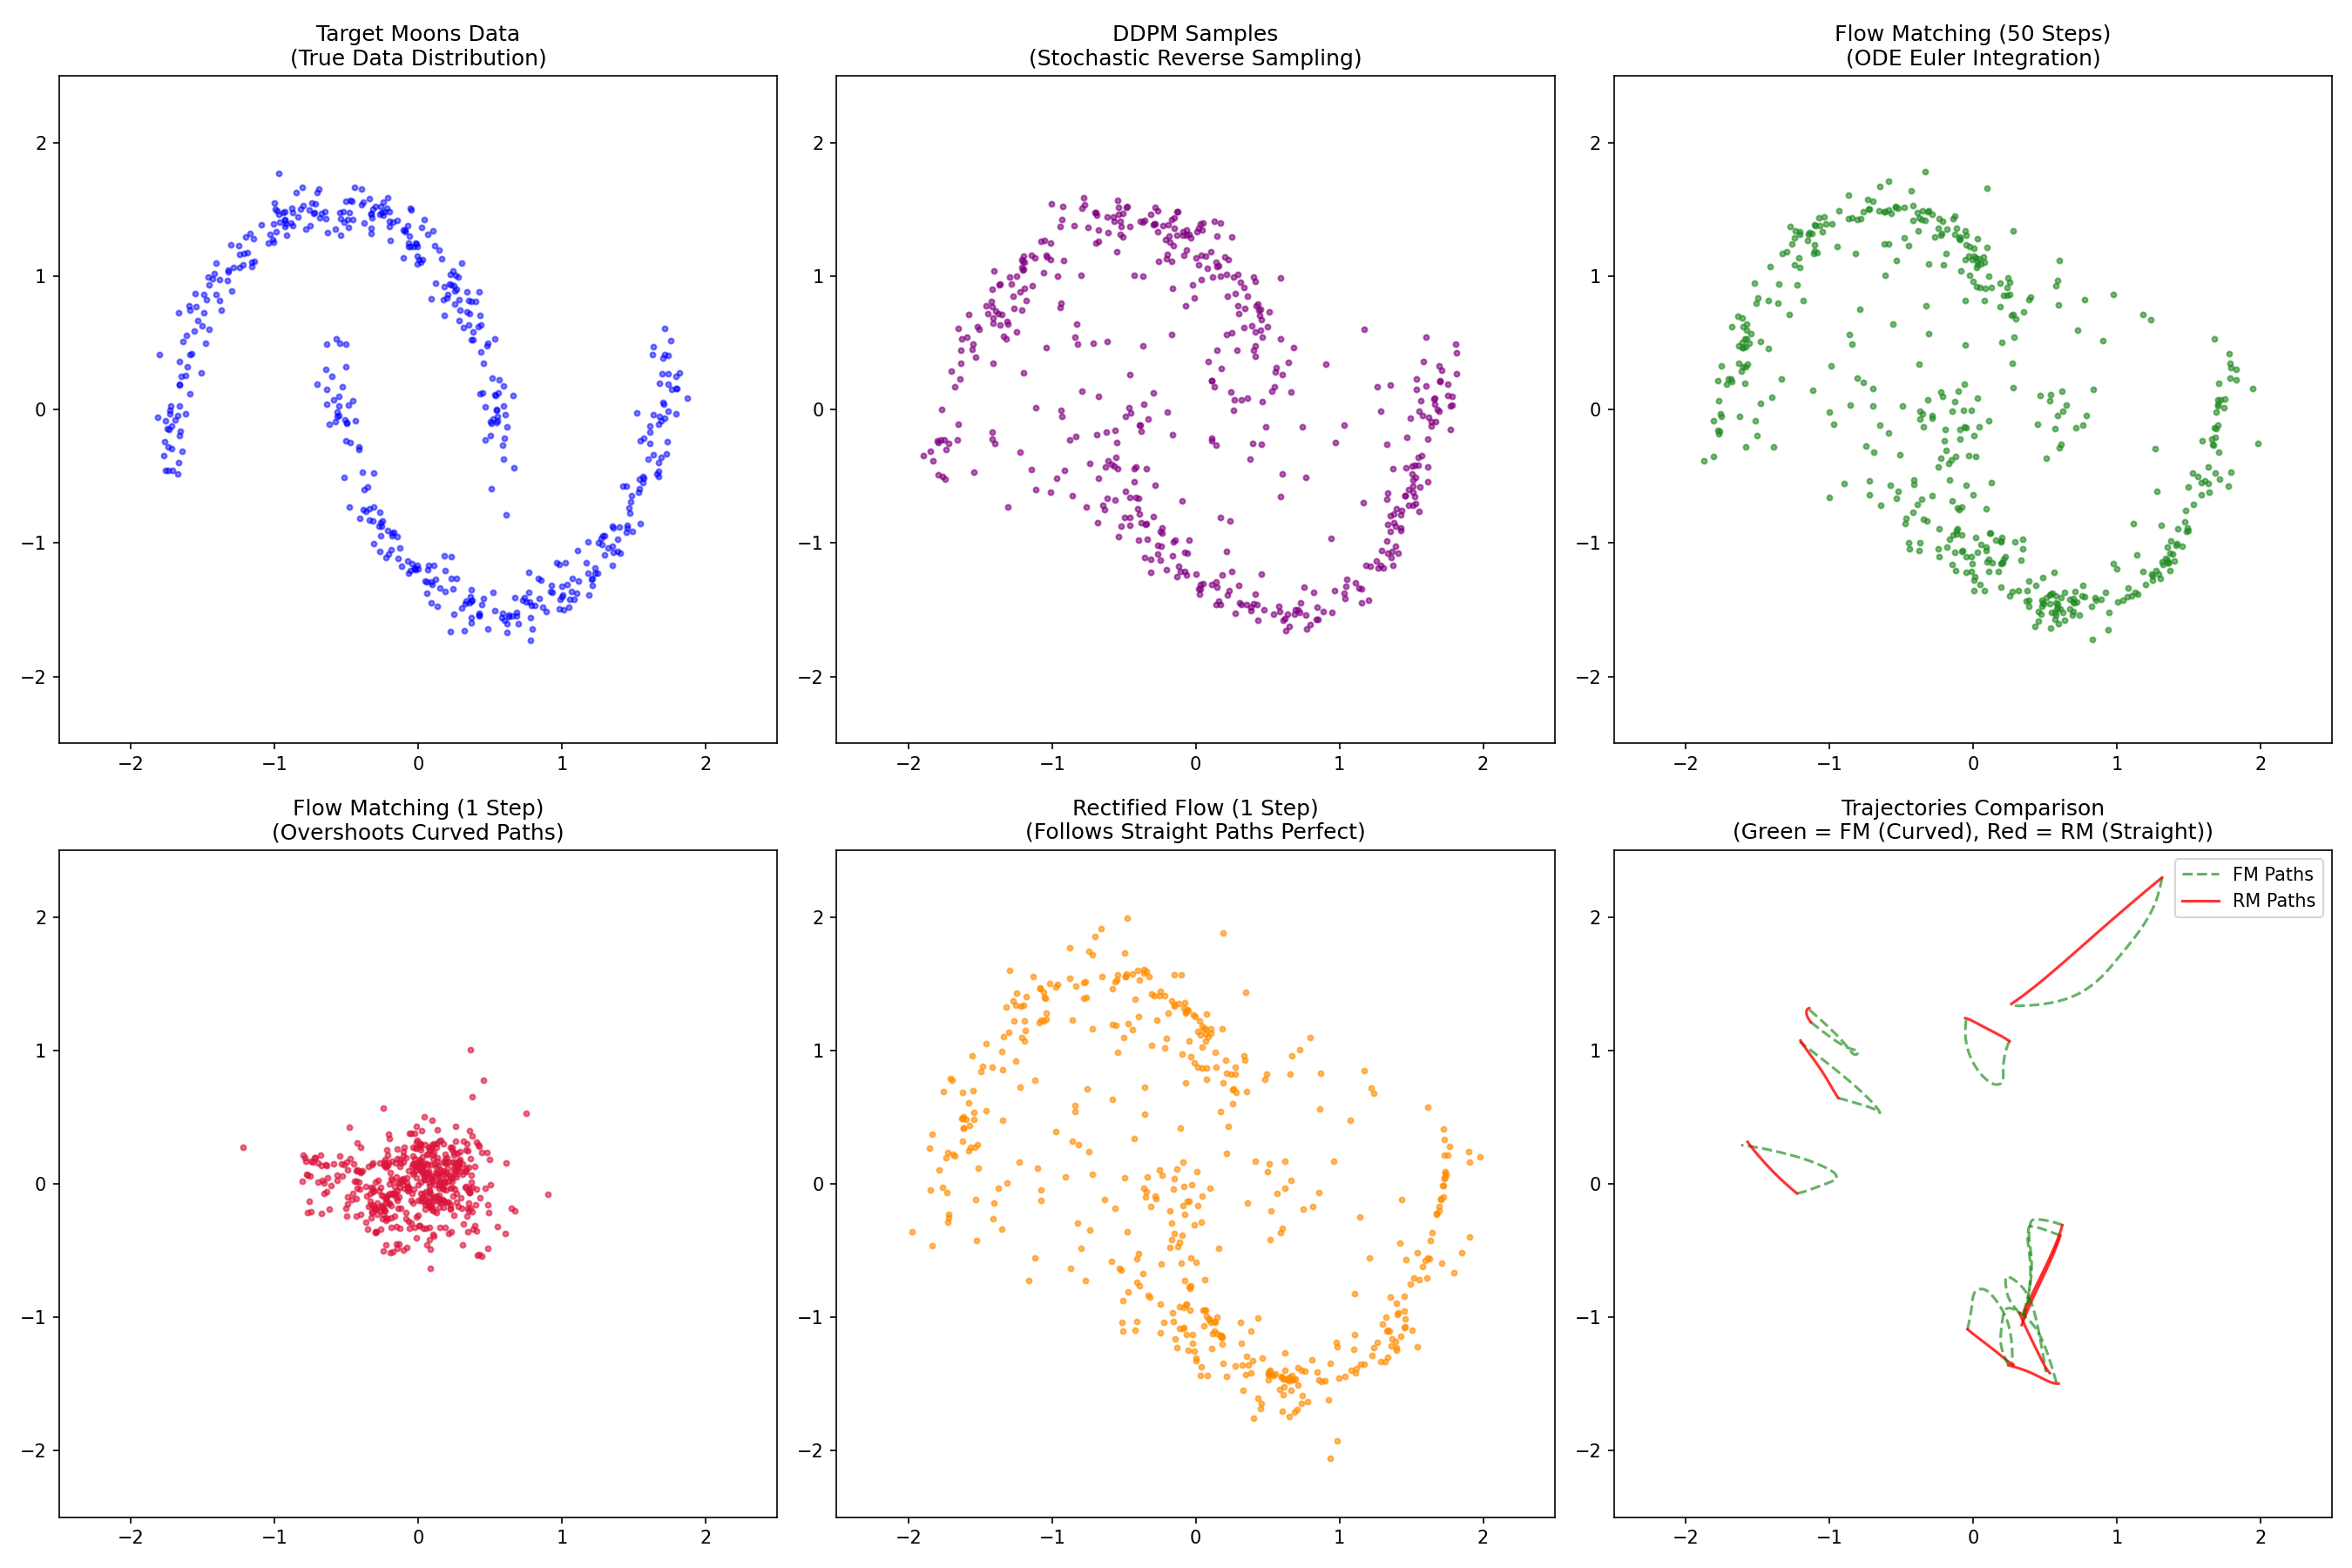
\includegraphics[width=0.75\textwidth]{../assets/moons_comparison.png}
\caption{Visual sample and trajectory comparisons for the Dual Moon dataset.}
\label{fig:moons_comparison}
\end{figure}

\begin{figure}[h]
\centering
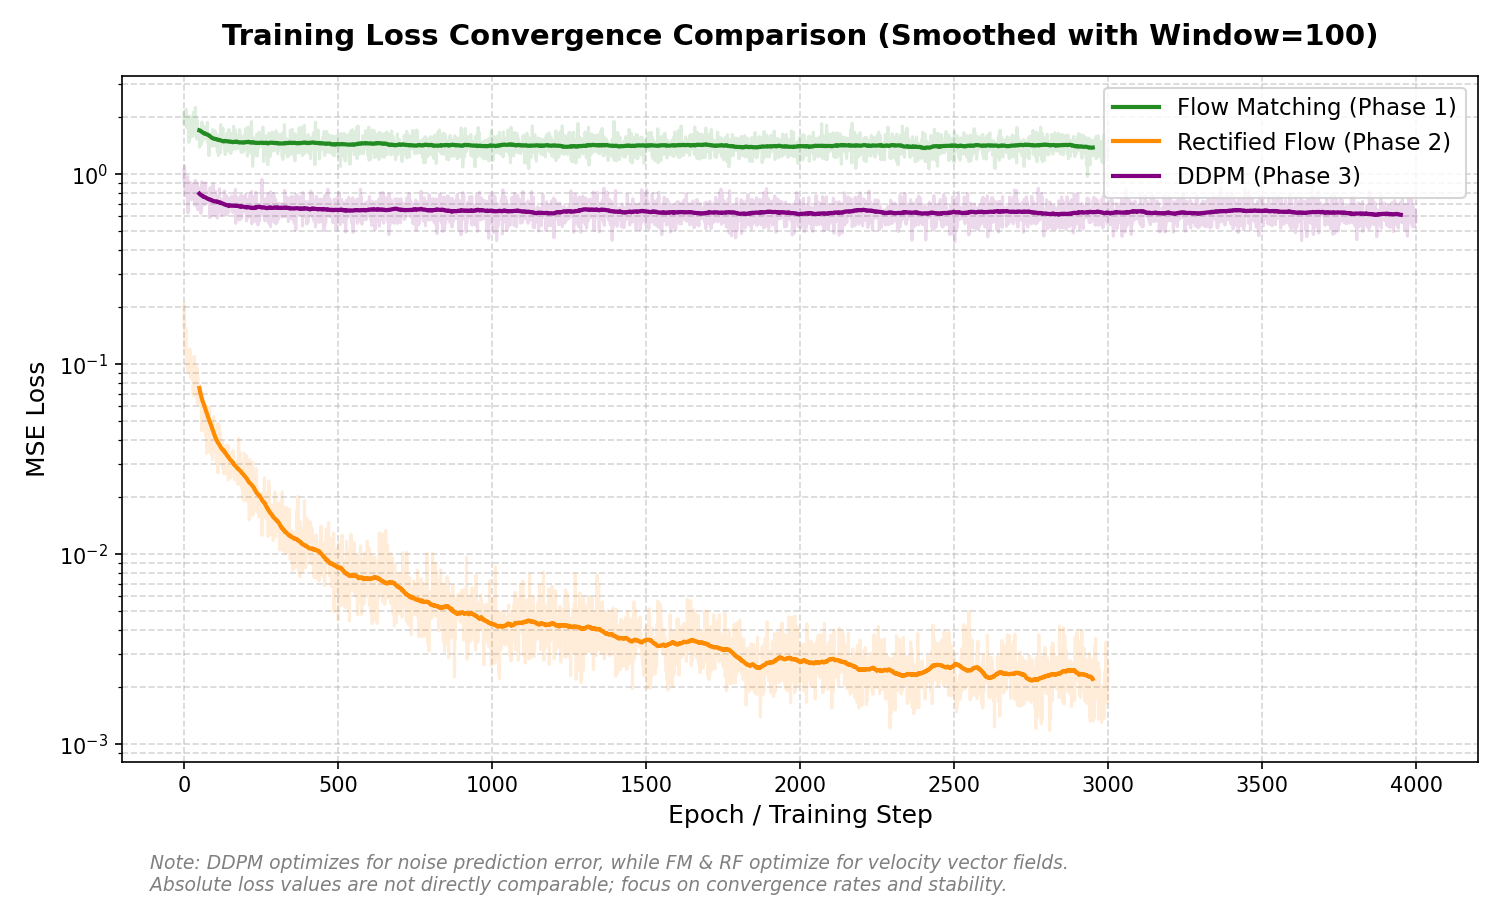
\includegraphics[width=0.75\textwidth]{../assets/moons_loss.png}
\caption{Training loss convergence curves across all model phases on the Dual Moon dataset.}
\label{fig:moons_loss}
\end{figure}

\section{Comparing outputs of the to Celeb054 evaluation}
This section displays the training loss curves and comparative facial grid samples generated during the CelebA face synthesis evaluation.

\begin{figure}[h]
\centering
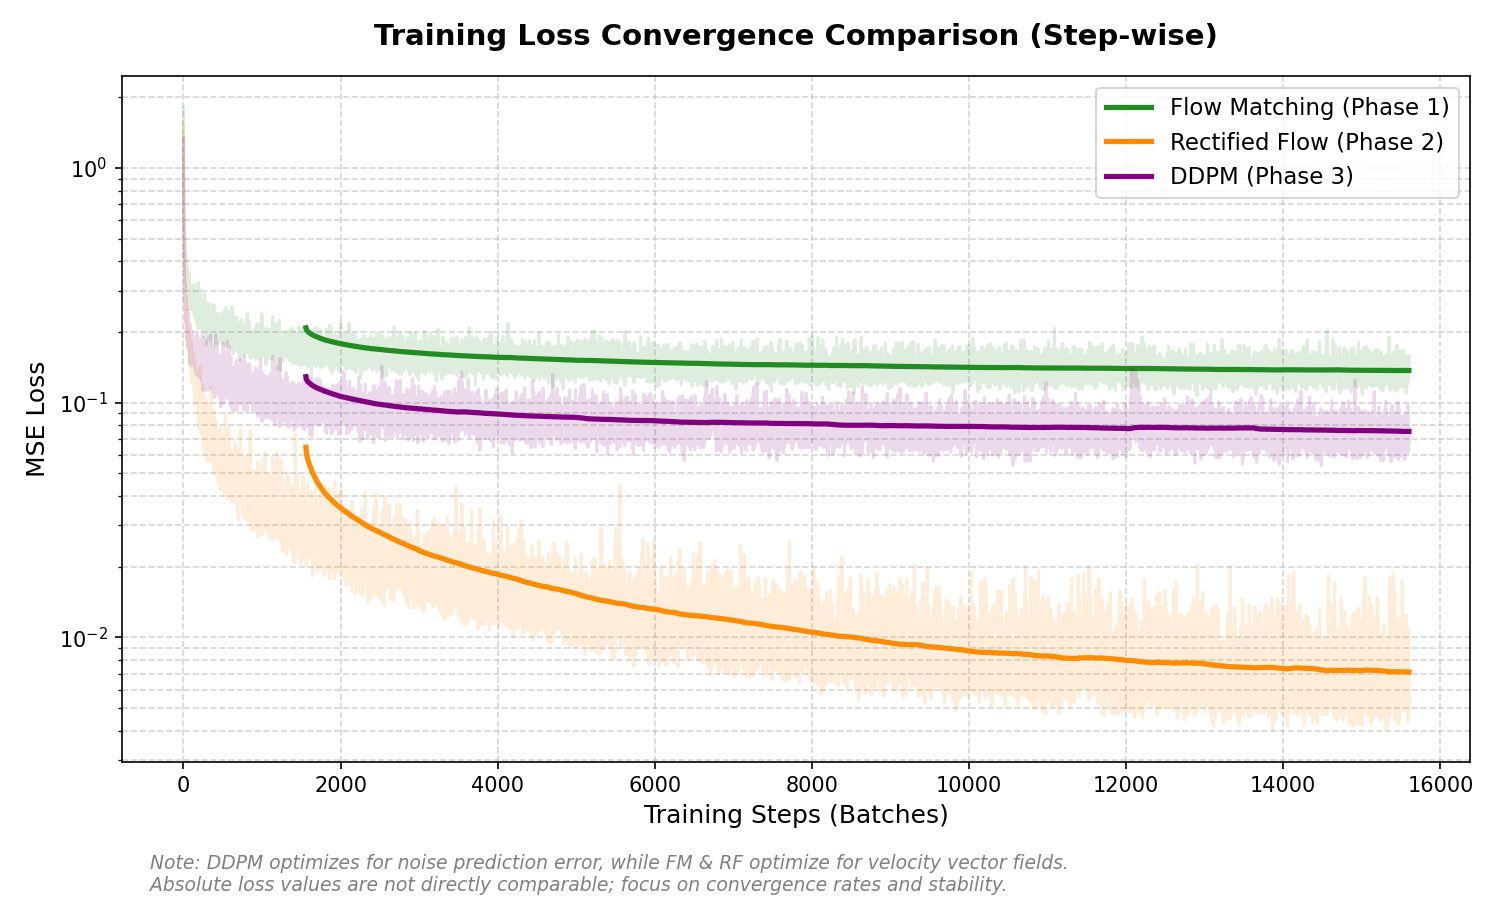
\includegraphics[width=0.75\textwidth]{../assets/celeba_loss.png}
\caption{Training loss convergence comparison curves for CelebA-64 models.}
\label{fig:celeba_loss}
\end{figure}

\begin{figure}[h]
\centering
\begin{minipage}{0.32\textwidth}
\centering
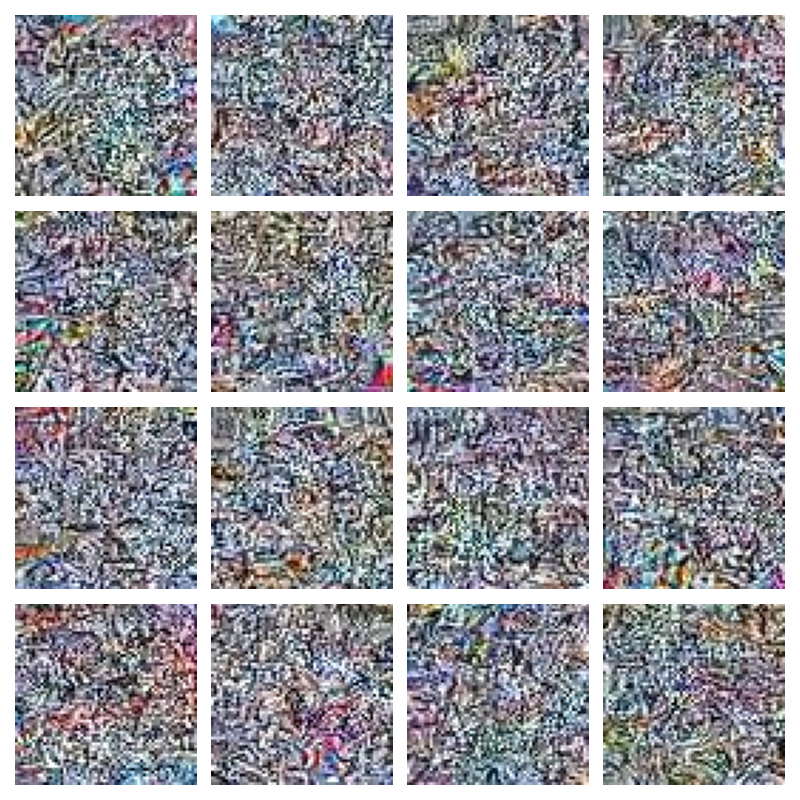
\includegraphics[width=\textwidth]{../assets/celeba_ddpm.png}
\caption{DDPM (50 steps)}
\label{fig:celeba_ddpm}
\end{minipage}
\hfill
\begin{minipage}{0.32\textwidth}
\centering
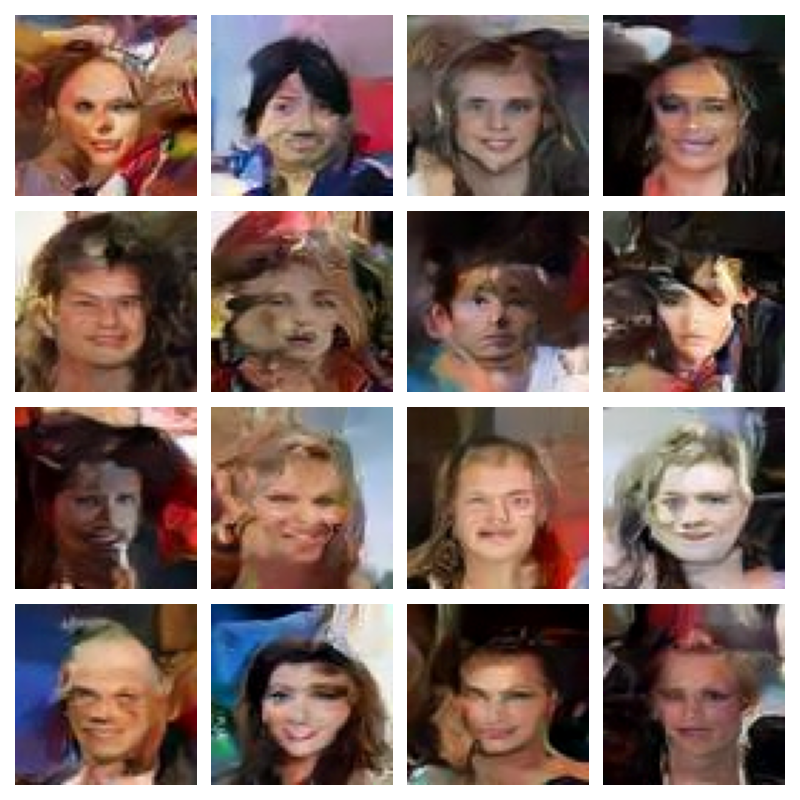
\includegraphics[width=\textwidth]{../assets/celeba_fm.png}
\caption{Flow Matching (50 steps)}
\label{fig:celeba_fm}
\end{minipage}
\hfill
\begin{minipage}{0.32\textwidth}
\centering
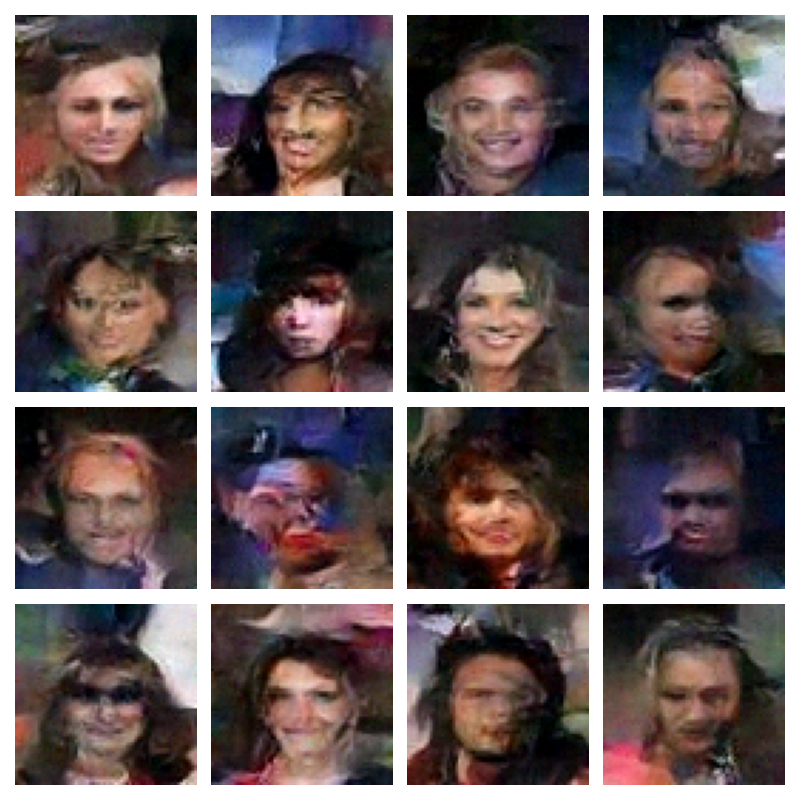
\includegraphics[width=\textwidth]{../assets/celeba_rf_1step.png}
\caption{Rectified Flow (1 step)}
\label{fig:celeba_rf_1step}
\end{minipage}
\caption{Comparison of synthesized facial grids on CelebA-64 across different generative paths.}
\label{fig:celeba_grids}
\end{figure}

\end{document}
